\documentclass[11pt,american,czech,oneside]{book}
    \usepackage[a4paper]{geometry}

    \usepackage[T1]{fontenc}
    \usepackage[utf8]{inputenc}
    \usepackage{babel}
    \usepackage{amsmath,amssymb,amsfonts,amsthm}
    \usepackage{indentfirst}
    \usepackage{graphicx}

    \usepackage{tikz}
    \usepackage{caption,lipsum}
    \usepackage{listings}
    \usepackage{mathtools}
    \usepackage{multirow}
    \usepackage{url}
    \usetikzlibrary{calc}

\theoremstyle{plain}
    \newtheorem{theorem}{Věta}
    \newtheorem{lemma}{Lemma}
    \newtheorem{proposition}{Tvrzení}
    \newtheorem*{corollary}{Důsledek}
\theoremstyle{definition}
    \newtheorem{definition}{Definice}
    \newtheorem{remark}{Poznámka}
    \newtheorem{example}{Příklad}
    \newtheorem{observation}{Pozorování}
\renewcommand*{\proofname}{Důkaz}

\newcommand{\TODO}[1]{\textcolor{red}{TODO: #1}\PackageWarning{TODO:}{#1!}}

\begin{document}

%----------------------------------------------------------------------

\chapter{Grafy, stromy} \TODO{nejaky hezky obrazky?} 
V této kapitole definujeme graf jakožto matematickou strukturu, popíšeme základní pojmy týkající se grafů a nastíníme možné vztahy mezi grafem a maticí. Dále definujeme strom, jakožto speciální případ grafu. Terminologie je převzata z \cite{koub:11}

\section{Základní grafová terminologie}

\begin{definition}
  Mějme množinu $V$ a množinu $E = \left\{ \left\{ u,v \right\} | u,v \in V \right\}$. Uspořádanou dvojici $G := (V,E)$, nazveme neorientovaný graf. Množinu $V$ nazýváme množinou vrcholů grafu $G$, jejím prvkům říkáme vrcholy, množinu $E$ nazýváme množinou hran grafu $G$, jejím prvkům říkáme hrany. Prvky hrany $e$ označujeme jako vrcholy incidentní hraně $e$ nebo koncové body hrany $e$. Říkáme, že hrana $e = \{v,w\}$ spojuje vrcholy $v$ a $w$.
\end{definition}

Pokud neuvažujeme hrany jako nejvýše dvouprvkové množiny vrcholů, ale  jako uspořádané dvojice $(u,v)$, nazýváme odpovídající graf \textbf{orientovaný}. Obvykle uvažujeme orientované a neorientované grafy zvlášť, ale je možné uvažovat i jejich kombinaci. Graf, v němž se vyskytují jak orientované tak neorientované hrany, nazýváme \textbf{smíšený}. Řekneme, že neorientovaný graf $G$ je \textbf{úplný}, pokud $\forall u, v \in V$ $\left(\{u,v\} \in E\right)$.

Povšimněme si, že v definici grafu není vyloučen případ, kdy jsou oba koncové body hrany shodné. Hrana je pak jednoprvkovou množinou a nazýváme ji \textbf{smyčkou} v grafu.

\begin{remark}
  V neorientovaném grafu $G=(V,E)$ platí, že jeho množina hran $E$ je podmnožinou ${V \choose 2} \cup V$, kde $V \choose 2$ značí množinu všech dvouprvkových podmnožin množiny $V$. V orientovaném grafu $H=(W,F)$ je $F$ podmnožinou množiny $W \times W$, tj. všech uspořádaných dvojic vrcholů z $W$.
\end{remark}

\textbf{Stupněm vrcholu} $v \in V$ rozumíme počet vrcholů spojených s vrcholem $v$, značíme $d(v)$. Množinu všech vrcholů, které jsou v grafu $G$ spojeny s vrcholem $v$ značíme $\mathrm{adj}_G(v)$.

\begin{definition}
  \textbf{Podgrafem} grafu $G$ nazveme libovolný graf $H=(W,F)$ který splňuje: $W\subseteq V$, $F\subseteq E$ a všechny vrcholy incidentní hranám z $F$ náleží do $W$. Úplný podgraf grafu $G$ nazýváme \textbf{klikou} v grafu $G$. Podgrafem grafu $G$ \textbf{indukovaným} množinou vrcholů $W$ nazveme takový podgraf $G$, který obsahuje všechny hrany grafu $G$, jejichž oba koncové body náleží do $W$, značíme $G(W)$.
\end{definition}


[TODO Potrebuju ohodnoceny, vazeny?]
\begin{definition}
  Mějme graf $G=(V,E)$ a zobrazení $\omega:V \rightarrow \mathbb{R}$, resp. $c: E \rightarrow \mathbb{R}$. Přidáním zobrazení $\omega$, resp. $c$ ke~grafu $G$ dostaneme graf, který nazýváme \textbf{ohodnocený}, resp. \textbf{vážený} reálným ohodnocením.
\end{definition}

\begin{definition}
  [TODO doplnit definici cesty bez cyklu!, cyklu, delka cesty]
\end{definition}

Existuje-li mezi libovolnými dvěma vrcholy grafu cesta, řekneme, že graf je \textbf{souvislý}.
\textbf{Vzdáleností} dvou vrcholů v souvislém grafu $G=(V,E)$ nazveme minimální délku cesty mezi těmito dvěma vrcholy. Vzdáleností vrcholu $v \in V$ od množiny vrcholů $W \subset V$ nazveme minimální vzdálenost mezi vrcholem $v$ a libovolným vrcholem náležícím do $W$. 

[TODO potrebuju bipartitni?]
[TODO potrebuju ctvercovou sit?]
[TODO potrebuju faktorgraf?]

\section{Strom}

Nyní zaveďme základní pojmy týkající speciální třídy grafů nazývané stromy \cite{koub:11}

\begin{definition}
  \textbf{Stromem} $T=(V,E)$ nazveme konečný souvislý neorientovaný graf bez cyklů. Pokud navíc v grafu $T$ vyznačíme bod $r \in V$, nazýváme uspořádanou dvojici $(T,r)$ \textbf{kořenovým stromem} a bod $r$ nazveme kořenem tohoto stromu.
\end{definition}

Z definice stromu je patrné, že každý vrchol $v$ kořenového stromu $(T,r)$ spojuje s kořenem tohoto stromu právě jedna cesta.
Vrcholy ležící na této cestě nazveme \textbf{předchůdci} vrcholu $v$. Předchůdce vrcholu $v$ různé od $v$ nazýváme \textbf{vlastními předchůdci} vrcholu $v$. Vrcholy, jejichž předchůdcem je vrchol $v$, nazýváme \textbf{následníky} vrcholu $v$. Vrcholy bez následníků nazýváme \textbf{listy stromu} $T$, vrcholy alespoň s jedním následníkem nazýváme \textbf{vnitřní vrcholy} stromu.

\begin{definition}
  \textbf{Podstromem} stromu $T$ určeným vrcholem $v$ nazveme indukovaný podgraf stromu $T$ tvořený vrcholem $v$ a a všemi jeho následníky.
\end{definition}

\section{Vztah grafu a matice}
\label{GrMatRel}
Grafy a matice spolu úzce souvisí, což nám umožňuje převádět problémy na maticích na problémy na grafech a naopak. Nezanedbatelným praktickým důsledkem jejich vzájemného vztahu je i možnost používat grafové algoritmy při řešení některých maticových úloh, především může být tento přístup výhodný pro řídké matice. Dělení grafů může posloužit například při snaze o paralelizaci rozkladu matice.

Neorientovaný graf $G=(V,E)$ s vrcholy $V = {v_1, \ldots, v_m}$ a hranami $E = {e_1, \ldots, e_n}$ Tento graf lze reprezentovat pomocí matice dvěma základními způsoby. \textbf{Maticí sousednosti}, neboli adjacenční matici, nazveme matici $A_G$ o rozměrech $m \times m$, jejíž prvek na pozici $(i,j)$ je definován jako:
\[
  {(A_G)}_{i,j} :=
  \left\{
    \begin{array}{@{\,}ll}
      1  & \mbox{existuje-li hrana spojující vrcholy $v_i, v_j$} \\
      0  & \mbox{jinak}
    \end{array}
  \right.
\]

 \textbf{Maticí incidence} grafu $G$ nazveme matici o rozměrech $m \times n$  definovanou následovně:
\[
  {(\bar{A}_G)}_{i,j} :=
  \left\{
	  \begin{array}{@{\,}ll}
		  1  & \mbox{je-li $v_i$ koncovým vrcholem hrany $e_j$} \\
		  0  & \mbox{jinak}
	  \end{array}
  \right.
\]

V kapitole ref{spektral} [TODO bude ref spektral?] budeme potřebovat \textbf{Laplaceovu matici} $Q$ grafu $G$, která je definována následovně:
\[
Q_{ij} :=
\left\{
	\begin{array}{@{\,}ll}
		-1  & \mbox{pro } i \neq j, (v_i,v_j) \in E \\
		0 & \mbox{pro } i \neq j, (v_i,v_j) \notin E\\
        d(i) & \mbox{pro } i = j
	\end{array}
\right.
\]
Laplaceovu matici $Q$ lze tedy vyjádřit jako $Q = D - A_G$, kde $D$  značí diagonální matici se stupni jednotlivých vrcholů na diagonále.

Pokud chceme reprezentovat matici pomocí grafu, většinou nám stačí zachytit její strukturu. V takovém případě můžeme pro popis obecně nesymetrické matice $A$ o rozměrech $n \times n$ použít orientovaný graf s množinou vrcholů $V = {v_1,\ldots,v_n}$ a množinou hran $E =\{(v_i,v_j)|a_{ij}\neq 0\}$. V případě, že je matice $A$ symetrická, můžeme ji analogickým způsobem reprezentovat pomocí neorientovaného grafu.
Pokud bychom chtěli do grafu zanést i numerické hodnoty jednotlivých prvků matice, museli bychom použít ohodnocený graf.

\begin{remark}
  Pro jednoduchost zaveďme následující terminologii. Říkáme, že graf $G$ \textbf{odpovídá} matici $A$ právě tehdy, když matice $A$ je maticí sousednosti grafu $G$.
\end{remark}

[TODO rozhodnout, jestli tam tohle dávat]
Pro reprezentaci ne nutně čtvercové matice $B$ o rozměrech $m\times n$ můžeme také použít bipartitní graf $G=(R,B,E)$ pro nějž platí $|R|=m$, $|B|=n$ a $E = \{(i,j') \ | \ i \in R, j' \in B, a_{ij} \neq 0 \}$.
[end TODO]

\bigskip
{
  \label{MatGrPicture}
  \centering
  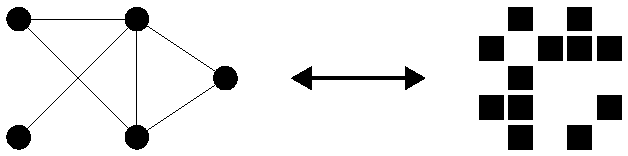
\includegraphics[width=0.7\textwidth]{pictures/matgr.pdf}
  \captionof{figure}{Příklad grafu a jemu odpovídající struktury matice\label{prGrMat}}
}

%----------------------------------------------------------------------

\chapter{Dělení grafů}
[TODO doplnit]

%----------------------------------------------------------------------

\chapter{Rozklady matic}
[TODO doplnit]

%----------------------------------------------------------------------

\chapter{Další parametry pro dělení grafu}
[TODO doplnit]

%----------------------------------------------------------------------

\chapter{Různé}
[TODO rozdistribuovat]
\section{Číslování}
\subsection{Číslování vrcholů grafu v závislosti na vzdálenosti od separátoru}
\label{sepDistNumbering}

    V této podkapitole popíšeme nejjednodušší metodu číslování vrcholů podgrafu, který vznikl rozdělením původního grafu na $n$ částí.
    Tuto metodu lze používat samostatně, ale vzhledem k její povaze ji lze využít i pro vylepšení ostatních metod očíslování grafu,
    například ji lze kombinovat s metodou minimálního stupně.

    Mějme graf $G = (V,E)$ a jeho vrcholový separátor [TODO znaceni], jehož odebráním se graf rozpadne na $n$ podgrafů $G_1, \ldots, G_n$.
    Popišme číslování vrcholů podgrafu $G_i$:

    \begin{enumerate}
      \item Položme $\texttt{j := 1}$.
      \item \label{sepDistAlg2} Nalezneme neočíslovaný vrchol $v$ grafu $G_i$ takový, že jeho vzdálenost od vrcholového separátoru v grafu $G$ je maximální.
      \item Tomuto vrcholu dáme číslo $\texttt{j}$, položíme $\texttt{j := j + 1}$.
      \item Pokud jsou všechny vrcholy očíslovány, skončíme, jinak se vrátíme na krok \ref{sepDistAlg2}
    \end{enumerate}

    Z algoritmu je vidět, že výsledné očíslování vrcholů grafu nemusí být jednoznačné, protože pokud nalezneme dva nebo více vrcholů, jejichž vzdálenost
    od separátoru je shodná, můžeme je očíslovat v libovolném pořadí.

\subsection{Číslování vrcholů pomocí metody minimálního stupně}
Metoda minimálního stupně je jednoduchým algoritmem pro nalezení očíslování grafu.
Algoritmus pro hledání očíslování grafu pomocí této metody je následující:

\begin{enumerate}
  \item Mějme graf $G=(V,E)$ a položme $j:=1$.
  \item \label{mindegloop}
      Nalezneme neočíslovaný vrchol $v$ grafu $G$ s nejmenším stupněm a přiřadíme mu číslo $j$.
  \item Přidáme hrany mezi vrcholy z $\mathrm{adj}_G(v)$ tak, aby $\mathrm{adj}_G(v)$ byla klika v grafu $G$.
  \item Pokud nejsou všechny vrcholy očíslované, zvětšíme $j$ o $1$ a vrátíme se na krok \ref{mindegloop}.
\end{enumerate}

Očíslování vrcholů grafu G pomocí tohoto algoritmu není jednoznačné, protože vrcholů s minimálním stupněm může být více.

Pokud máme rozdělení $G_1, \ldots, G_n$ grafu $G$ s vrcholovým separátorem [TODO znaceni], můžeme pro očíslování části $G_i$ použít
číslování vrcholů pomocí metody minimálního stupně, kde při výběru vrcholu ve \ref{mindegloop}. kroku přidáme kritérium vzdálenosti od separátoru
popsané v \ref{sepDistNumbering}. Nejprve tedy nalezneme množinu všech vrcholů grafu $G$, které mají minimální stupeň
a poté mezi nimi zvolíme ten, který má nejmenší stupeň.

\subsection{Topologické číslování vrcholů stromu}
\begin{definition}
    Mějme graf $G = (V,E)$, který je stromem. Očíslování jeho vrcholů nazveme topologickým právě tehdy,
    když pro každý vrchol $v \in V$ platí, že libovolný následník vrcholu $v$ ve stromu $G$ má nižší číslo než vrchol $v$.
\end{definition}

\section{Další témata}
[TODO Řídké matice vs. husté matice]


%----------------------------------------------------------------------

\chapter{Eliminační stromy}
V této kapitole se budeme zabývat eliminačními stromy a jejich významem pro rozklady řídkých matic.
Eliminační stromy při rozkladu matic hrají důležitou roli, protože nám dávají informaci o zaplnění
v Choleského faktoru matice bez toho, abychom museli počítat jednotlivé numerické hodnoty.
Lze tedy díky nim jednoduše porovnávat vhodnost zvoleného uspořádání řádků a sloupců matice pro Choleského rozklad.

V této kapitole bez újmy na obecnosti předpokládáme, že matice, jejíž Choleského rozklad chceme napočítávat, je ireducibilní,
a tedy přidružený graf této matice je souvislý.

\section{Definice eliminačního stromu matice}

Nejprve se omezme na ireducibilní, pozitivně definitní, symetrickou matici $A_T$ o rozměrech $n \times n$,
jejíž přidružený graf $G(A_T)$ je strom. V tomto případě je $A_T$ tzv. perfektní eliminační matice, tj. existuje permutační matice $P$ taková,
že Choleského rozklad matice $PA_TP^T$ nebude obsahovat žádné zaplnění \cite{rose:72}
(Matici $PA_TP^T$ můžeme vnímat pouze jako přečíslování řádků a sloupců matice $A_T$).
Aby při choleského rozkladu matice $A_T$ nedošlo k žádnému zaplnění, stačí když pomocí topologického číslování očíslujeme vrcholy jí přidruženého grafu (z předpokladu se jedná o strom)
a řádky a sloupce matice $A_T$ seřadíme odpovídajícím způsobem. Pak zjevně platí, že matice $A_T$ má, s výjimkou posledního řádku,
pod diagonálou vždy právě jeden nenulový prvek.
Díky tomu můžeme definovat pro matici $A_T$ funkci $\texttt{PARENT}: \{1,\ldots,n\} \rightarrow {1,\ldots,n}$ následovně:
\begin{align*}
  \forall j \in \{1,\ldots,n-1\} \quad \texttt{PARENT}[j] & := p \quad \Leftrightarrow \quad a_{p,j} \neq 0 \wedge p > j \\
  \text{a speciálně:} \quad \texttt{PARENT}[n] & := 0.
\end{align*}
Zřejmě ve stromu přidruženém k matici $A_T$ platí, že předchůdcem vrcholu $x_j$ je vrchol $x_{\texttt{PARENT}[j]}$.

Většinou však nepracujeme s maticemi, jejichž přidružený graf by byl stromem. Zavedeme tedy konstrukci pro libovolnou
řídkou, ireducibilní, pozitivně definitní, symetrickou matici $A$ o rozměrech $n \times n$.
Předpokládejme, že známe Choleského rozklad této matice, tj. $A = LL^T$. Maticí se zaplněním nazveme matici $F$ definovanou jako $F = L + L^T$.
Dále zavedeme matice $L_t$ a $F_t$ následovně. $L_t$ je matice vzniklá z $L$ tím, že v každém sloupci vynulujeme všechny prvky pod diagonálou
kromě prvku s nejnižším řádkovým indexem a $F_t = L_t L_t^T$.

Z definice $F_t$ vidíme, že se jedná o matici, jejíž přidružený graf $G(F_t)$ je strom.

\begin{definition}
    Eliminačním stromem matice $A$ nazveme graf $G(F_t)$ popsaný výše, značíme $T(A)$.
    Podstrom $T(A)$ s kořenem $x_j$ značíme $T[x_j]$. Množinu vrcholů tohoto stromu značíme také $T[x_j]$.
\end{definition}

Díky této definici můžeme definici funkce $\texttt{PARENT}$ přirozeně rozšířit na matici $A$ následovně:
\[
    \texttt{PARENT}[j] := \min \{i > j | l_{i,j} \neq 0\},
\]
kde $l_{i,j}$ označuje $i,j$-tý prvek matice $L$.

\begin{observation}
Přímo z definice plyne, že $T(A)$ a $T(F)$ jsou identické.
\end{observation}

\begin{observation}
Pokud $x_i$ je vlastním předchůdcem $x_j$ v eliminačním stromu, pak $i > j$.
\end{observation}

\begin{proposition}
  Pro $i>j$ závisí numerické hodnoty sloupce $L_{\bullet i}$ na sloupci $L_{\bullet j}$ právě tehdy,
  když $l_{i,j} \neq 0$.
\end{proposition}
\begin{proof}
  Tvrzení plyne přímo ze sloupcového algoritmu [???]
\end{proof}

%----------------------------------------------------------------------

\chapter{Algoritmizace a implementace}

Cílem programu, který jsme implementovali, je ukázat, že rozdělení grafu získané za pomoci profesionální numerické knihovny pro dělení grafů METIS, nemusí být vyvážené vzhledem k výpočtu Choleského rozkladu na vzniklých oblastech. Dále jsme se pokusili navrhnout a otestovat metodu přerozdělení grafu založenou na přečíslování vrcholů grafu. Cílem navržené metody je zlepšit rozdělení grafu tak, aby počet operací potřebných pro Choleského faktorizaci na jednotlivých oblastem byl pokud možno stejný a nebyl vyšší než maximum z počtu operací při rozdělení počátečním.

[TODO Fortran, Fortran90, c++]
[TODO dělení na kolik částí?]

Naši implementaci můžeme rozdělit na několik logických celků. [TODO doplnit]

\section{Formát a uložení vstupní matice}
V této podkapitole bude popsán vstupní formát matice a způsob její reprezentace v našem programu.
[TODO Zajímá nás jen struktura]

\subsection{Vstupní formát matice}

Jako základní matice pro testování výsledků našeho programu nám posloužily matice uložené ve formátu RSA v souborech s příponou \texttt{.rsa} nebo \texttt{.rb}. Jako zdroj pro tyto matice jsme použili kolekci \cite{hbcol}.

[TODO popis HB formátu]

Pro testování jsme dále používali matice vygenerované při jednoduché pětibodové diskretizaci dvojrozměrné Poissonovy rovnice (podprogram \texttt(poisson)) a několik jednoduchých testovacích matic, které jsme si ručně zapsali do souboru \texttt{testing.f90}

\subsection{Reprezentace matice v programu}

Matice je v našem programu uložena v \textbf{CSR formátu} (compressed sparse row format) \cite{pis:84,saad:94}, který je běžně využívaným formátem sloužícím pro reprezentaci řídkých matic a grafů. 

Mějme řídkou matici $A$ o rozměrech $n \times n$, která obsahuje $n_e$ nenulových prvků. Tuto matici v programu reprezentujeme pomocí tří polí: pole \texttt{ia} o délce $n+1$ a polí \texttt{ja},\texttt{aa} o délce $n_e$. V poli \texttt{ja} na pozicích \texttt{ia($i$)},\ldots,\texttt{ia($i+1$)-1} jsou uloženy sloupcové indexy nenulových prvků na $i$-tém řádku matice $A$, na odpovídajících pozicích v poli \texttt{aa} jsou uloženy numerické hodnoty těchto prvků.

\begin{example}
  \label{CSRexample}
  Mějme následující symetrickou matici
  \[
    \begin{pmatrix}
      0 & 5 & 0 & 3 & 0 \\
      5 & 0 & 9 & 4 & 2 \\
      0 & 9 & 0 & 0 & 0 \\
      3 & 4 & 0 & 0 & 4 \\
      0 & 2 & 0 & 4 & 0
    \end{pmatrix}
  \]
  Pak její reprezentace ve formátu CSR vypadá následovně:
  \begin{verbatim}
    ia = [ 1, 3, 7, 8, 11, 13 ]
    ja = [ 2, 4, 1, 3, 4, 5, 2, 1, 2, 5, 2, 4 ]
    aa = [ 5, 3, 5, 9, 4, 2, 9, 3, 4, 4, 2, 4 ]
  \end{verbatim}
\end{example}

Pokud budeme uvažovat pouze pole \texttt{ia}, \texttt{ja}, je podle teorie popsané v oddíle \ref{GrMatRel} výsledná reprezentace matice $A$ zároveň reprezentací neorientovaného grafu, kterému matice $A$ odpovídá. Pokud tedy nebudeme brát v úvahu hodnoty jednotlivých prvků matice, můžeme při popisu implementace bez újmy na obecnosti pojmy graf a matice zaměňovat.

\begin{example}
  Vezměme matici z příkladu \ref{CSRexample}. Pak graf, který je reprezentován pomocí polí \texttt{ia}, \texttt{ja} je zobrazen na obrázku \ref{MatGrPicture}
\end{example}

\section{Knihovna METIS pro dělení grafu}

Pro samotné dělení grafu jsme využili knihovnu pro dělení grafů METIS \cite{kary:13} verze 5.1.0.

Vzhledem k tomu, že jsme dělení grafů používali jako nástroj pro vyvažování počtu operací při Choleského rozkladu na jednotlivých oblastech, potřebovali jsme nalézt rozdělení grafu pomocí vrcholového separátoru. Takové rozdělení nám poskytne rutina \texttt{METIS\_ComputeVertexSeparator}, kterou jsme ve Fortranu implementovali pomocí rozhraní \texttt{metis\_interface.f95} a \texttt{metisinclude.c}. 

\section{Softwarové požadavky pro běh}
Pro úspěšné slinkování a zkompilování
[TODO nainstalovaný METIS]






%----------------------------------------------------------------------

\chapter*{Závěr}
[TODO doplnit]


\newpage
\bibliographystyle{plain}
\bibliography{diplomka}

\end{document} 